\section{Preliminaries} \label{sec:preliminaries}
\subsection{High dimensional expanders}
Most of the definitions in this subsection are standard, with the exception of the definition of the non-lazy up down walk \pref{def:non-lazy-up-down}.

A pure \(d\)-dimensional simplicial complex \(X\) is a hypergraph that consists of an arbitrary collection of sets of size \((d+1)\) together with all their subsets. The sets of size \(i+1\) in \(X\) are denoted by \(X(i)\). The vertices of \(X\) are denoted by \(X(0)\) (we identify between a vertex \(v\) and its singleton \(\set{v}\)). We will sometimes omit set brackets and write for example \(uvw\in X(2)\) instead of \(\set{u,v,w}\in X(2)\). As a convention \(X(-1) = \set{\emptyset}\).
%
Let \(X\) be a pure \(d\)-dimensional simplicial complex. Let \(k \leq d\). We denote the set of oriented \(k\)-faces in \(X\) by \(\dir{X}(k) = \sett{(v_0,v_1,...,v_k)}{\set{v_0,v_1,...,v_k} \in X(k)}\).

For \(k \leq d\) we denote by \(X^{\leq k} = \bigcup_{j=-1}^k X(j)\) the \(k\)-skeleton of \(X\). When \(k=1\) we call this complex \emph{the underlying graph of \(X\)}, since it consists of the vertices and edges in \(X\) (as well as the empty face).

A \emph{clique complex} is a simplicial complex such that if \(s \subseteq X(0)\) has that if \(s\) is a clique, that is, for every two vertices \(v,u \in s\) the edge \(vu \in X(1)\), then \(s \in X\).

A \((d+1)\)-partite \(d\)-dimensional simplicial complex is a generalizeation of a bipartite graph. It is a complex \(X\) such that one can decompose \(X(0) = A_0 \dunion A_1 \dunion \dots \dunion A_d\) such that for every \(s \in X(d)\) and \(i \in \set{0,\ldots,d}\) it holds that \(\abs{s \cap A_i} = 1\).

\subsubsection*{Probability over simplicial complexes}
Let \(X\) be a simplicial complex and let \(\Pr_d:X(d)\to (0,1]\) be a density function on \(X(d)\) (that is, \(\sum_{s \in X(d)}\Pr_d(s)=1\)). This density function induces densities on lower level faces \(\Pr_k:X(k)\to (0,1]\) by \(\Pr_k(t) = \frac{1}{\binom{d+1}{k+1}}\sum_{s \in X(d),s \supset t} \Pr_d(s)\). We can also define a probability over directed faces, where we choose an ordering uniformly at random. Namely, for \(s\in \dir{X}(k)\), \(\Pr_k(s) = \frac{1}{(k+1)!}\Pr_k(set(s))\) (where \(set(s)\) is the set of vertices participating in \(s\)). When clear from the context, we omit the level of the faces, and just write \(\Pr[T]\) or \(\Prob[t \in X(k)]{T}\) for a set \(T \subseteq X(k)\).

\subsubsection*{Links in a high dimensional expander} Let \(X\) be a \(d\)-dimensional simplicial complex and let \(s \in X\) be a face. The link of \(s\) is the \(d'=d-|s|\)-dimensional complex
\[X_s = \sett{t \setminus s}{t \in X, t \supseteq s}.\]
For a simplicial complex \(X\) with a measure \(\Pr_d:X(d) \to (0,1]\), the induced measure on \(\Pr_{d',X_s}:X_s(d-|s|)\to (0,1]\) is
\[\mathbb{P}_{d',X_s}(t \setminus s) = \frac{\Pr_d(t)}{\sum_{t' \supseteq s} \Pr_d(t')}.\]

We denote by \(\lambda(X_s)\) the (normalized) second largest eigenvalue of the adjacency operator of \(X_s^{\leq 1}\). We denote by \(\abs{\lambda}(X_s)\) to be the (normalized) second largest (in absolute value) eigenvalue of the adjacency operator of \(X_s^{\leq 1}\).

\begin{definition}[High dimensional expander]
    Let \(X\) be a \(d\)-dimensional simplicial complex and let \(\lambda \in (0,1)\). We say that \(X\) is a \emph{\(\lambda\)-one sided high dimensional expander} if for every \(s \in X^{\leq d-2}\) it holds that \(\lambda(X_s) \leq \lambda\). We say that \(X\) is a \emph{\(\lambda\)-two sided high dimensional expander} if for every \(s \in X^{\leq d-2}\) it holds that \(\abs{\lambda}(X_s) \leq \lambda\).
\end{definition}
We stress that this definition includes \(s= \emptyset\), which also implies that \(X^{\leq 1}\) itself should have a small second largest eigenvalue.

\subsubsection*{Walks on high dimensional expanders}
Let \(X\) be a \(d\)-dimensional simplicial complex. Let \(\ell \leq k \leq d\). The \((k,\ell)\)-containment graph \(G_{k,\ell}=G_{k,\ell}(X)\) is the bipartite graph whose vertices are \(L=X(k), R=X(\ell)\) and whose edges are all \((t,s)\) such that \(t \supseteq s\). The probability of choosing such an edge is by choosing \(t \sim X(k)\) and a uniform \(s \subseteq t\) of size \(\ell+1\).

\begin{theorem}[\cite{KaufmanO2020}] \label{thm:eignevalues-of-walk}
    Let \(X\) be a \(d\)-dimensional \(\lambda\)-one sided high dimensional expander. Let \(\ell \leq k \leq d\). Then the second largest eigenvalue of \(G_{k,\ell}(X)\) is upper bounded by \(\lambda(G_{k,\ell}(X)) \leq \frac{\ell+1}{k+1} + O(k\lambda)\).
\end{theorem}

A corollary proven in \cite{DinurK2017} is that this graph is also a good sampler.
\begin{corollary}[\cite{DinurK2017}] \label{cor:good-sampler-from-expansion}
    Let \(A \subseteq X(k)\), \(\ell \leq k\) and \(\zeta > 0\). Let
    \[B(A) = \sett{s \in X(\ell)}{\Abs{\Prob[t\supseteq s]{A} - \prob{A}} > \zeta}.\]
    Then \(\prob{B(A)} = O(\frac{\ell+1}{(k+1) \zeta^2}\prob{A})\).
\end{corollary}

A related walk is the swap walk. Let \(k,\ell,d\) be integers such that \(\ell+k\leq d-1\). The \(k,\ell\)-swap walk \(S_{k,\ell}=S_{k,\ell}(X)\) is the bipartite graph whose vertices are \(L=X(k), R=X(\ell)\) and whose edges are all \((t,s)\) such that \(t \dunion s \in X\) (and in particular \(t,s\) are disjoint). The probability of choosing such an edge is the probability of choosing \(u \in X(k+\ell+1)\) and then uniformly at random partitioning it to \(u=t\dunion s\). This walk has been defined and studied independently by \cite{DiksteinD2019} and by \cite{AlevFT2019}, who bounded its spectral expansion.

\begin{theorem}[\cite{DiksteinD2019,AlevFT2019}]
    Let \(X\) be a \(\lambda\)-two sided high dimensional expander. Then the second largest eigenvalue of \(S_{k,\ell}(X)\) is upper bounded by \(\lambda(S_{k,\ell}(X)) \leq (k+1)(\ell+1)\lambda\).
\end{theorem}

We also define another random walk call the non-lazy up down walk.
\begin{definition}[Non lazy up down walk] \label{def:non-lazy-up-down}
    Let \(X\) be a \(d\)-dimensional simplicial complex. Let \(d_1\leq d_2 \leq d\) such that \(2d_1 \geq d_2-1\). The \((d_1,d_2)\)-non lazy up down walk is the distribution \((s_1,s_2) \sim DU_{n}\) of \(X(d_1)\) where \(s_1,s_2\) are chosen by first choosing \(t \in X(d_2)\) and then uniformly sampling \(s_1,s_2 \in X(d_1)\) such that \(s_1 \cup s_2 = t\).
\end{definition}
The reason this is called non-lazy, is because we do not allow \(s_1 \cup s_2 \subsetneq t\) as in the usual up-down walk defined in \cite{DiksteinDFH2018} for example. We note that \(\Abs{s_1 \cap s_2} = 2d_1-d_2+1\), i.e. the intersection size doesn't depend on the pair chosen. We can decompose this walk also as sampling \(r= s_1 \cap s_2 \in X(2d_1-d_2)\), then sampling \(p_1,p_2 \in X_r(d_2-d_1)\) according to the swap walk, and then outputting \(s_1 = r \cup p_1, s_2 = r \cup p_2\).

\subsubsection*{The spherical building}
Let \(d \in \NN\) and \(q\) be a prime power. 
\begin{definition}\label{def:sph-bldg}
    The spherical building (sometimes called the \(SL_d(\mathbb{F}_q)\)-spherical building), is the complex \(X\) whose vertices are all non-trivial linear subspaces of \(\mathbb{F}_q^d\). Its higher dimensional faces are all flags \(\sett{W_0 \subseteq W_1 \subseteq \dots \subseteq W_m}{W_0,W_1,\dots,W_m \subseteq \mathbb{F}_q^d}\). 
\end{definition}
This complex is \((d-2)\)-dimensional.

\begin{claim}[\cite{EvraK2016}] \label{claim:spherical-building-hdxness}
    Let \(X\) be a \(SL_d(\mathbb{F}_q)\)-spherical building. Then \(X\) is a \(O(\frac{1}{\sqrt{q}})\)-one sided high dimensional expander. Moreover, \(X^{\leq k}\) is a \(\max \set{O(\frac{1}{\sqrt{q}}), \frac{1}{d-k}}\)-two sided high dimensional expander.
\end{claim}

\subsection{Agreement tests} \label{sec:agreement-tests}

Let \(k<d\) and let \(X\) be a \(d\)-dimensional simplicial complex. Let \(\Sigma\) be some fixed alphabet and suppose we have an ensemble of functions \(\mathcal{F} = \sett{f_r:r\to \Sigma}{r \in X(k)}\).% 

An two-query agreement test is a distribution \(\mathcal{D}\) over pairs \(r_1,r_2 \in X(k)\). The agreement of an ensemble is
\begin{equation}
    \agr_{\mathcal{D}}(\mathcal{F}) = \Prob[r_1,r_2\sim \mathcal{D}]{f_{r_1} = f_{r_2}}.
\end{equation}
When we write \(f_{r_1} = f_{r_2}\) we mean that \(f_{r_1}(v)=f_{r_2}(v)\) for every \(v \in r_1 \cap r_2\).

More generally, a \(q\)-ary agreement test is a distribution of \(r_1,r_2,...,r_q \in X(k)\), where the agreement of the ensemble
\begin{equation}
    \agr_{\mathcal{D}}(\mathcal{F}) = \Prob[r_1,r_2,\dots r_q \sim \mathcal{D}]{\forall i,j \; f_{r_i} = f_{r_j}}.
\end{equation}

Let \(\Delta_k(d)\) be the \(k\)-dimensional complete complex over \(d\) vertices. Let \(\mathcal{D}\) be a \(q\)-ary agreement test on \(\Delta_k(d)\) and assume that it is symmetric\footnote{i.e. for every permutation \(\pi:[d] \to [d]\) it holds that \(\prob{s_1,s_2,...,s_q} = \prob{\pi(s_1),\pi(s_2),...,\pi(s_q)}.\)}. Let \(X\) be another \(d\)-dimensional simplicial complex. We define the \emph{extension} \(\mathcal{D}_X\) of \(\mathcal{D}\) to an agreement test on \(X\), as follows:
\begin{enumerate}
    \item Sample \(t \in X(d)\).
    \item Query \(r_1,r_2,...,r_q \subseteq t\) according to \(\Delta_k(d)\).
\end{enumerate}
We note that by the symmetry of \(\mathcal{D}\) the second step doesn't depend on the way we identify the vertices of \(t\) with the vertices of \(\Delta_k(d)\). Let us give two examples for such tests, that were considered in previous works. %
\begin{definition}[Two-query \(V\)-test]
    Let \(d = 2k-\sqrt{k+1}+1\).
    \begin{enumerate}
        \item Sample some \(t \in X(d)\).
        \item Sample uniformly \(s_1,s_2 \in X(k)\) such that \(s_1, s_2 \subseteq t\), conditioned on \(\abs{s_1 \cap s_2} = \sqrt{k+1}\).
    \end{enumerate}
\end{definition}

\begin{definition}[Three-query \(Z\)-test]
    Let \(d=3k-2\sqrt{k+1}+2)\).
    \begin{enumerate}
        \item Sample some \(t \in X(d)\).
        \item Sample three \(s_1,s_2,s_3 \in X(k)\) such that \(s_1, s_2, s_3 \subseteq t\), conditioned on \(\abs{s_1 \cap s_2}, \abs{s_2 \cap s_3} = \sqrt{k+1}\) and \(s_1 \cap s_3 = \emptyset\).
    \end{enumerate}
\end{definition}

%
A sound distribution is a distribution that supports an agreement theorem.
\begin{definition} \label{def:distribution-soundness}
    Let \(X\) be a simplicial complex and let \(\mathcal{D}\) be an agreement distribution on \(X\). Let \(\eta,\varepsilon_0,e > 0\) be constants. We say that \(\mathcal{D}\) is \emph{\((\eta,\varepsilon_0,e)\)-sound} if for every ensemble of functions \(\mathcal{F}\) such that \(\agr_{\mathcal{D}}(\mathcal{F}) = \varepsilon \geq \varepsilon_0\), there exists a function \(G:X(0)\to \Sigma\), such that
    \begin{equation} \label{eq:dist-soundness}
        \Prob[r_1,r_2,\dots,r_q \sim \mathcal{D}]{\forall j \; G|_{r_j} \overset{1-\eta}{\approx} f_{r_j} \ve \forall i,j \; f_{r_i} = f_{r_j}} \geq \frac{1}{2}\varepsilon^e.    
    \end{equation}
    
\end{definition}
Here \(f \overset{1-\eta}{\approx} g\) means that \(f,g\) differ on at most a \(\eta\)-fraction of their coordinates, or stated differently \(\dist(f,g) \leq \eta\).

We extend this definition to soundness with respect to covers in \pref{def:distribution-cover-soundness}, after we introduce simplicial covers formally.

Here are some examples of such distributions.
\begin{example} \label{ex:sound-distributions}
    \begin{enumerate}
    \item Dinur and Goldenberg showed that the \(V\)-test extended to \(X=\Delta_k(n)\) is \((\sqrt{k},k^{-c},1)\)-sound for \(d \geq k^3\)  and \(c > 0\) \cite{DinurG2008}\footnote{In fact, \cite{DinurG2008} considered a \(V\)-test with a smaller intersection size, but the same result hold for \(\sqrt{k}\) too. See \cite{ImpagliazzoKW2012} for a proof for the intersection size of \(\sqrt{k}\).}.
    \item The \(1\%\)-agreement theorem by Impagliazzo, Kabanets and Wigderson, showed that the \(Z\)-test extended to \(X=\Delta_k(n)\) together with the techniques used in \cite[Theorem 5.1]{DinurG2008} show that the \(Z\)-test is \((k^{-0.2},exp(-\Omega(k^{1/2}),O(1))\)-sound.
    \item Dinur and Livni-Navon, together with the techniques used in \cite[Theorem 5.1]{DinurG2008} show that the \(Z\)-test is \((\lambda,exp(-\Omega(k)),O(1))\)-sound for every constant \(\lambda > 0\) \cite{DinurL2017}.
\end{enumerate}
\end{example}

Here \(n \gg k\) in all cases. We remark that the exact distributions in the works in the example were not described the way we described them (the conditioning in the second step required the intersection to be at least a certain size, not exactly a certain size). However, when the complex is large enough the TV-distance between the distributions in all previous works, and the distributions we described above, is negligible in the regime of parameters we consider. We therefore ignore this small point.

We also stress that while previous works give very strong agreement results, that apply for \(\varepsilon_0 = \exp(-\Omega(k))\), our technique currently yields results on for \((\eta,\varepsilon_0,O(1))\) such that \(\eta \exp(\poly(1/\varepsilon)) \ll 1\), so in particular, we will always think of \(\varepsilon = 1/\log(k)\) in the main theorem.

\subsection{Covering maps}
In this subsection we give a short introduction to covers and their connection to \(1\)-cohomology. We stress that everything we state in this subsection is well known. For a more in depth discussion, see \cite{Surowski1984}.

\begin{definition}[Covering map]\label{def:cover}
    Let \(Y,X\) be simplicial complexes. We say that a map \(\rho:Y(0) \to X(0)\) is a covering map if the following holds.
    \begin{enumerate}
        \item \(\rho\) is a surjective homomorphism.
        \item For every \(v \in X(0)\), and \((v,i) \in \rho^{-1}(\set{v})\) it holds that \(\rho|_{Y_{(v,i)}}:Y_{(v,i)}(0) \to X_v(0)\) is an isomorphism.
    \end{enumerate}
    We often denote \(\rho:Y\to X\). We say that \(\rho\) is an \(\ell\)-cover if for every \(v \in X(0)\) it holds that \(\Abs{\rho^{-1}(\set{v})}=\ell\). If there exists such a covering map \(\rho:Y\to X\) we say that \(Y\) covers \(X\).
\end{definition}

Let us see two examples for covers.
\begin{example} \label{ex:trivial-cover}
    Let \(X\) be any simplicial complex. Let \(Y\) be \(\ell\)-disconnected copies of \(X\). Then the projection of every to \(X\), \(\rho:Y \to X\), is a covering map. This cover a called the trivial cover.
\end{example}

\begin{figure}
    \centering
    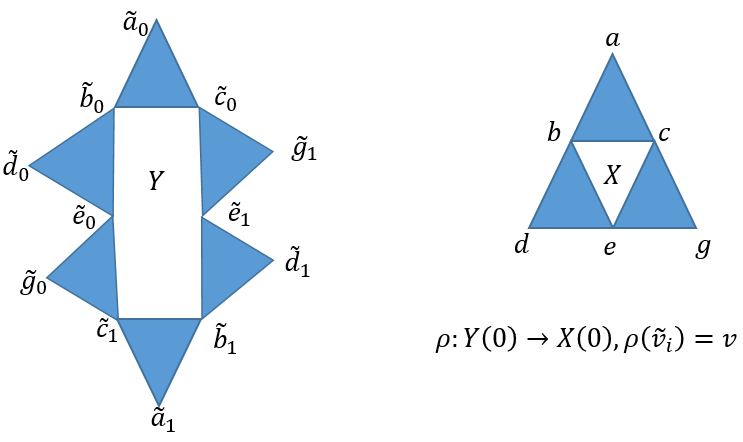
\includegraphics[scale=0.5]{images/cover_example.png}
    \caption{Non trivial connected cover}
    \label{fig:cover-example}
\end{figure}
\begin{example}
    \pref{fig:cover-example} contains an example of a \(\rho:Y \to X\) such that \(Y\) is connected.
\end{example}
Next we develop some basic properties of covers that are both necessary for our result, and give some intuition of the structure of covers.

The first property we show is that a cover \(\rho:Y \to X\) induces a permutations \(\pi_{uv}\) for every directed edge \(uv \in \tilde{X}(1)\) that ``encode'' the covers information as in the claim below.
\begin{claim} \label{claim:permutations-from-covers}
    Let \(X\) be a simplicial complex and let \(\rho:Y \to X\) be a cover. Let \(vu \in \dir{X}(1)\). Let \(\rho^{-1}(v) = \set{(v,1),(v,2),\dots,(v,\ell)}\) and \(\rho^{-1}(u) = \set{(u,1),(u,2),\dots,(u,\ell')}\). Then \(\ell = \ell'\) and there exists \(\pi_{uv}:[\ell]\to [\ell]\) such that \(\pi_{uv}(i)=j\) if and only if \(\set{(v,i), (u,j)} \in Y(1)\).
\end{claim}

Using these permutations we can show that all covers of a connected simplicial complex are \(\ell\)-covers.
\begin{corollary} \label{cor:every-cover-is-regular}
    If \(X\) is connected then any cover of \(X\) is an \(\ell\)-cover for some \(\ell \in \NN \cup \set{\infty}\).
\end{corollary}

\begin{proof}[Proof of \pref{claim:permutations-from-covers}]
    First we note that for every \((v,i)\) there is a unique \((u,j)\) such that \(\set{(v,i), (u,j)} \in Y(1)\). This is because \(\rho|_{\tilde{X}_{(v,i)}}:X_{(v,i)}(0)\to X_v(0)\) is an isomorphism so there is a single preimage of \(u\) in \(X_{(v,i)}(0)\). Hence there are functions \(\pi_{uv}:[\ell] \to [\ell']\) and \(\pi_{uv}:[\ell'] \to [\ell]\) such that \(\pi_{uv}(i)=j\) if and only if \(\set{(v,i), (u,j)} \in Y(1)\). These functions invert each other from their definition, i.e. \(\pi_{uv}(i)=j\) if and only if \(\set{(v,i), (u,j)} \in Y(1)\) if and only if \(\pi_{vu}(j)=i\) hence \(\ell=\ell'\) and this is the required permutation.
\end{proof}

\begin{proof}[Proof of \pref{cor:every-cover-is-regular}]
    Let \(X\) be a connected complex and assume that there exists a cover \(\rho:Y\to X\) such that \(Y\) is not an \(\ell\)-cover for any \(\ell\). Let \(\ell\) be the number of images of some arbitrary vertex \(v \in X(0)\). Let \(B = \sett{v' \in X(0)}{\Abs{\rho^{-1}(v')} = \ell} \ne \emptyset\). If \(X(0) \setminus B\) is not empty then the cut between \(B\) and \(X(0) \setminus B\) has an edge crossing it. But the number of preimages for both sides of the edge is equal which lead to a contradiction.
\end{proof}

Finally, let us show that in an \(\ell\)-cover, every \(s \in X\) has \(\ell\)-inverse images.
\begin{claim} \label{claim:inverse-image-of-l-cover}
    Let \(\rho:Y \to X\) be an \(\ell\)-cover. Then for every non-empty \(s \in X\),
    \[\abs{\rho^{-1}(s)} = \ell.\]
\end{claim}

\begin{proof}[Proof of \pref{claim:inverse-image-of-l-cover}]
    Let \(s \in X\). Let \(v \in s\) be any vertex inside \(s\) and we write \(s = \set{v} \dunion r\). By definition, there are \(\ell\)-vertices \((v,1),(v,2),\dots,(v,\ell)\) such that \(\rho((v,i)) = v\). By the local isomorphism property between \(X_v\) and every \(Y_{(v,i)}\), there are faces \(\tilde{r}_i \in Y_{(v,i)}\) such that \(\rho(\tilde{r}_i) = r\). The faces \(\tilde{s}_i = \tilde{r}_i \dunion \set{(v,i)}\) are \(\ell\)-inverse images of \(s\). This shows that \(\abs{\rho^{-1}(s)} \geq \ell\). Let us see that every preimage of \(s\) it one of these \(\tilde{s}_i\). Indeed, let \(\hat{s} \in \rho^{-1}(s)\). Let \((v,i) \in \hat{s}\) be the preimage of \(v\) in \(\hat{s}\). Then \(\hat{r} = \hat{s} \setminus \set{(v,i)} \in Y_{(v,i)}\) maps to \(r\). By the fact that \(\rho|_{Y_{(v,i)}}:Y_{(v,i)}(0) \to X_v(0)\), this implies that \(\hat{r}=\tilde{r}_i\). Thus \(\hat{s}= \tilde{s}_i\).
\end{proof}

\subsubsection{The induced function}
Let \(\rho:Y \to X\) be an \(\ell\)-cover. Without loss of generality we identify 
\[Y(0) = X(0) \times [\ell] = \sett{(v,i)}{v \in X(0), \; i=1,2,\dots,\ell}\]
where \(\rho((v,i)) = v\). We define \emph{the induced function} 
\begin{equation} \label{eq:induced-function}
    \psi_{\rho}:\dir{X}(1) \to Sym(\ell), \; \psi_{\rho}(vu)=\pi_{uv}
\end{equation}
where \(\pi_{uv}(i)=j\) are such that \(\set{(v,i), (u,j)} \in Y(1)\) (as in \pref{claim:permutations-from-covers}). The first thing we notice is that this function is asymmetric, i.e., \(\psi(uv)=\psi(vu)^{-1}\) for every edge \(uv \in \dir{X}(1)\). Let 
\[C^1(X,Sym(\ell)) = \sett{\psi:\dir{X}(1)\to Sym(\ell)}{f \text{ is asymmetric}}\]
be the space of asymmetric functions. These functions are sometimes referred to as non-abelian cochains in the literature. One may suspect if there is a bijection between covers \(\rho\) and \(\psi \in C^1(X,Sym(\ell))\), but there are many \(\psi \in C^1(X,Sym(\ell))\) whose permutations don't give rise to a cover. It turns out that and asymmetric function \(\psi \in C^1(X,Sym(\ell))\) corresponds to a cover if and only if for every triangle \(uvw \in \dir{X}(2)\) it holds that \begin{equation} \label{eq:cover-condition}
    \psi_{\rho}(vw) \circ \psi_{\rho}(uv)=\psi_{\rho}(uw).
\end{equation}
We denote by \(Z^1(X,Sym(\ell)) \subseteq C^1(X,Sym(\ell))\) 
\[ Z^1(X,Sym(\ell)) = \sett{\psi \in  C^1(X,Sym(\ell))}{\forall uvw \in \dir{X}(2), \; \psi(vw) \circ \psi(uv)=\psi(uw)}.\]

\begin{claim} \label{claim:necessary-conditionfor-covers}
    Let \(\rho:Y \to X\) be an \(\ell\)-cover. Then \(\psi_{\rho} \in Z^1(X,Sym(\ell))\).
\end{claim}

\begin{proof}[Proof of \pref{claim:necessary-conditionfor-covers}]
    Let \(\rho:Y \to X\) and fix \(uvw \in X(2)\), let us show that \(\psi_{\rho}(vw) \circ \psi_{\rho}(uv)=\psi_{\rho}(uw)\). Indeed, by definition \(\psi_{\rho}(xy) = \pi_{yx}\) where \(\pi_{yx}(i)=j\) if and only if \(\set{(x,i), (y,j)} \in Y(1)\). Indeed, let \(\pi_{uv}(i)=j\) and \(\pi_{wv}(i)=k\) and we need to show that \(\pi_{wu}(j)=k\), which is equivalent to showing that if \(\set{(v,i),(u,j)}, \set{(v,i),(w,k)} \in Y(1)\) then \(\set{(u,j),(w,k)} \in Y(1)\). \(\rho:Y_{(v,i)}(0) \to X_v(0)\) is an isomorphism, it holds that \(\set{(u,j), (w,k)} \in Y_{(v,i)}(1)\) and in particular the edge is in \(Y(1)\).
\end{proof}

If \(\psi \in Z^1(X,Sym(\ell))\), then we can construct a cover \(\rho=\rho_\psi:Y \to X\) such that \(\psi_{\rho} = \psi\) as follows.
\begin{definition} \label{def:induced-cover}
    Let \(\psi \in C^1(X,Sym(\ell))\) and denote by \(\psi(vu)=\pi_{uv}\). The induced cover is the complex \(Y=Y_\psi\) and mapping \(\rho_\psi:Y \to X\) defined by
    \begin{enumerate}
        \item \(Y(0) = X(0) \times [\ell]\) and \(\rho_\psi((v,i))=v\).
        \item \(Y(1) = \sett{\set{(v,i),(u,\pi_{uv}(i))}}{v \in X(0), vu \in \dir{X}(1), i \in [\ell]}\).
        \item \(\tilde{s}=\set{(v_0,i_0),(v_1,i_1),\dots, (v_m,i_m)} \in Y(m)\) if and only if \(s=\rho(\tilde{s})=\set{v_0,v_1,\dots,v_m} \in X(m)\) and for every \(v_{p},v_{q} \in s\) it holds that \(\pi_{v_q,v_p}(i_p)=i_q\).
    \end{enumerate}
\end{definition}

\begin{claim} \label{claim:reconstruction of a cover}
    Let \(\psi \in Z^1(X,Sym(\ell))\). Then \(\rho_\psi:Y \to X\) is an \(\ell\)-cover of \(X\) and \(\psi_{\rho}=\psi\).
\end{claim}

\begin{proof}[Proof of \pref{claim:reconstruction of a cover}]
It is obvious that \(\rho\) is surjective and that it is a homomorphism from the definition. Let \(v \in X(0)\) and \((v,i) \in Y(0)\). We show that \(\rho|_{Y_{(v,i)}(0)}:Y_{(v,i)}(0) \to X_v(0)\) is an isomorphism. First let us make sure that this is a bijection. By definition, for every edge \(\set{v,u} \in X(1)\) there is an edge \(\set{(v,i),(u,\pi_{uv}(i))} \in Y(1)\) so \(\rho|_{Y_{(v,i)}(0)}\) is surjective. A priori, there could have been more edges \(\set{(v,i),(u,k)}\) if \(i=\pi_{vu}(k)\), but because \(\psi\) is asymmetric, \(i=\pi_{vu}(k)\) implies that \(\pi_{uv}(i)=k\) so the restriction is also injective.

We continue by showing that this is an isomorphism. First note that this bijection is a homomorphism by definition (there are no faces \(\tilde{s} \in Y(m)\) unless their projection \(\rho(\tilde{s}) \in X(m)\), so the same holds for the link of \((v,i)\)). Thus it remains to show that for every \(s \in X_v(m)\) there is some \(\tilde{s} \in X_{(v,i)}(m)\) such that \(\rho(\tilde{s})=s\). By definition of the link, \(s \dunion \set{v}=t \in X(m+1)\). We will show that
\(\tilde{t}=\set{(v,i)} \dunion \sett{(u,j_u)}{u \in s, j_u=\pi_{uv}(i)}\) is in \(Y(m+1)\), which implies that \(\sett{(u,j_u)}{u \in s, j_u=\pi_{uv}(i)}=\tilde{s} \in Y_{(v,i)}(m)\) maps to \(s\).

As \(\rho(\tilde{t})=t\) this amounts to showing that all possible edges \(xy \in Y(1)\) for \(x,y \in \tilde{t}\). One case is when, say, \(x=(v,i)\) and \(y=(u,j_u)\). In this case, \(\set{(v,i),(u,\pi_{uv}(i))} \in Y(1)\) and \(\pi_{uv}(i)=j_u\) by definition, hence the \(xy \in Y(1)\). The other case is when \(x=(u,{j_u})\) and \(y=(w,{j_w})\) for some \(u,w \in s\). in this case we note that \(\pi_{uv}(i)=j_u, \pi_{wv}(i)=j_w\). By \eqref{eq:cover-condition} applied for \(vuw \in X(2)\), it holds that \(j_w=\pi_{wv}(i)=\pi_{wu}(\pi_{uv}(i))=\pi_{wu}(j_u)\). Hence \(\set{(u,{j_u}),(w,{j_w})} \in Y(1)\) and the statement is proven.

The fact that \(\psi_{\rho}=\psi\) follows directly from the definition of the edges in \(Y\).
\end{proof}

\subsubsection{Connectivity of covers}
A simply connected complex is a connected complex such that every cover looks like \pref{ex:trivial-cover}, i.e., a bunch of disconnected copies of the original complex.
\begin{definition}[simply connected complex]
    Let \(X\) be a connected simplicial complex. We say that \(X\) is \emph{simply connected} if it is connected and if for every \(\ell\)-cover \(\rho:Y \to X\) there exists a partition of \(Y\) to \(\ell\) disconnected components \(Y= Y_1 \dunion Y_2 \dunion ... \dunion Y_\ell\) such that \(\rho|_{Y_i}:Y_i \to X\) is an isomorphism.
\end{definition}

\subsubsection{Further properties of covers}
\begin{claim} \label{claim:restriction-of-cover}
Let \(\rho:Y \to X\) be an \(\ell\)-cover. Let \(A \subseteq X(0)\) and let \(X'\) be the induced subcomplex over the vertices of \(A\). Let \(Y'=\rho^{-1}(A)\). Then \(\rho|_{Y'}:Y' \to X'\) is an \(\ell\)-cover.
\end{claim}

\begin{proof}[Proof of \pref{claim:restriction-of-cover}]
    Let \(\psi \in Z^1(X,Sym(\ell))\) such that \(Y=X^\psi\) is the induced cover as in \pref{def:induced-cover}. Then \(\psi|_{X'(1)} \in Z^1(X',Sym(\ell))\) and \(\rho|_{Y'}\) is the induced cover of this restriction.
\end{proof}


\begin{claim}\label{claim:cover-of-clique-complex}
    Let \(X\) be a clique complex and let \(\rho:Y\to X\) be a cover of \(X\). Then \(Y\) is a clique complex.
\end{claim}

\begin{proof}[Proof of \pref{claim:cover-of-clique-complex}]
    Let \(\tilde{s} = \set{(v_0,i_0),(v_1,i_1),...,(v_k,i_k)} \subseteq Y(0)\) be clique. Thus \(\rho(\tilde{s}) = s \subseteq X(0)\) is also a clique, and thus \(s \in X(k)\), or equivalently \(s \setminus \set{v_0} \in X_{v_0}(k-1)\). The link of \(v_0\) in \(X\) is isomorphic to the link of \((v_0,i_0)\) via \(\rho\). In particular this implies that \(\tilde{s} \setminus \set{(v_0,i_0)} \in Y_{(v_0,i_0)}(k-1)\) which is equivalent to \(\tilde{s} \in Y(k)\).
\end{proof}

\begin{claim} \label{claim:expansion-of-cover}
    Let \(X\) be a \(\lambda\)-one or two sided high dimensional expander. Then any connected cover is a \(\frac{\lambda}{1-\lambda}\)-one or two sided spectral expander respectively.
\end{claim}

The proof of this claim relies on the trickling down theorem by Oppenheim \cite{Oppenheim2018}.

\begin{theorem}[\cite{Oppenheim2018}] \label{thm:trickle-down}
    Let \(X\) be a \emph{connected} simplicial complex and assume that for any vertex \(v \in X(0)\) it holds that \(X_v\) is a \(\lambda\)-one or two sided high dimensional expander. Then the underlying graph of \(X\) is a \(\frac{\lambda}{1-\lambda}\)-one or two sided spectral expander (respectively), which implies that \(X\) is a \(\frac{\lambda}{1-\lambda}\)-one or two sided high dimensional expander (respectively).
\end{theorem}

\begin{proof}[Proof of \pref{claim:expansion-of-cover}]
    Let \(\rho:Y \to X\) be a cover such that \(Y\) is connected. For every vertex \(\tilde{v} \in Y\) such that \(\rho(\tilde{v})=v\), it holds that \(Y_{\tilde{v}} \cong X_v\). Thus in particular, if \(X\) is a \(\lambda\)-one or two sided high dimensional expander, this implies that \(Y_{\tilde{v}}\) is a \(\lambda\)-high dimensional expander. By \pref{thm:trickle-down}, \(Y\) is also a \(\frac{\lambda}{1-\lambda}\)-one or two sided high dimensional expander.
\end{proof}

\subsection[Cover soundness à la (CLA)]{Cover-soundness à la \pref{eq:CLA}}
Let us extend the definition of sound agreement tests to accommodate for our new notion of covers.
\begin{definition}[Cover sound] \label{def:distribution-cover-soundness}
    Let \(X\) be a simplicial complex and let \(\mathcal{D}\) be an agreement distribution on \(X\). Let \(\eta,\varepsilon_0,e > 0\) be constants. We say that \(\mathcal{D}\) is \emph{\((\eta,\varepsilon_0,e)\)-cover-sound} if for every ensemble of functions \(\mathcal{F} = \sett{f_r:r \to \Sigma}{r \in X(k)}\) such that \(\agr_{\mathcal{D}}(\mathcal{F}) = \varepsilon \geq \varepsilon_0\),
    there exists a simplicial $\frac{1}{\varepsilon^e}$-cover \(\rho:Y \to X\) and a global function \(G:Y(0)\to \Sigma\) such that 
    \begin{equation} \label{eq:dist-cover-soundness}
        \Prob[r \in Y(k)]{f_{\rho(r)}\circ \rho \overset{1-\eta}{\approx} G|_r} \geq \frac{1}{2}\varepsilon^e.
    \end{equation}
\end{definition}
The probability in \eqref{eq:dist-cover-soundness} is equivalent to choosing \(r \in X(k)\) and then a random preimage \(\tilde{r} \in Y(k)\). Therefore this inequality implies that for at least \(\frac{1}{2}\varepsilon^e\)-fraction of the \(f_r\)'s, the function agrees with \(G|_{\tilde{r}}\) for one of the preimages \(\tilde{r} \in \rho^{-1}(r)\) (i.e. using \(\rho\) to send vertices from \(\tilde{r}\) to \(r\)).

We note that here we did not require the cover to explain most of the agreement, but this definition actually implies such a statement. See discussion in \cite{DinurG2008} (there it is done for the complete complex, but their techniques are general).

\subsection{Cosystolic expansion and cover property testing}
Recall that \(Z^1(X,Sym(\ell)) \subseteq C^1(X,Sym(\ell))\) are all asymmetric functions such that \(\psi(uw)=\psi(vw)\circ \psi(uv)\) for every triangle \(uvw \in \dir{X}(2)\). For our result we will need simplicial complexes where this relation is locally testable. For this we define for every two function \(\psi,\phi: \dir{X}(k) \to Sym(\ell)\) their distance
\begin{equation} \label{eq:def-of-dist}
    \dist(\psi,\phi) = \Prob[s \in \dir{X}(k)]{\psi(s) \ne \phi(s)}.
\end{equation}
We also denote the weight of the function \(\wt(\psi) = \dist(\psi,Id)\) (where \(Id:\dir{X}(k) \to Sym(\ell)\) assigns every face \(s \in \dir{X}(k)\) the identity permutation).

For \(\psi \in C^1(X,Sym(\ell))\) we define \(\coboundary \psi: \dir{X}(2) \to Sym(\ell)\) by
\begin{equation} \label{eq:def-of-coboundary}
    \coboundary(\psi) = \psi(wu)\circ \psi(vw) \circ \psi(uv).
\end{equation}

We are ready to define cosystolic expansion.
\begin{definition} \label{def:def-of-cosyst-exp}
    Let \(X\) be a \(d\)-dimensional simplicial complex for \(d \geq 2\). Let \(\beta >0\). We say that \(X\) is a \(\beta\)-cosystolic expander if for every \(\ell \in \NN\), and every \(\psi \in C^1(X,Sym(\ell))\) there exists some \(\phi \in Z^1(X,Sym(\ell))\) such that
    \begin{equation} \label{eq:def-of-cosyst-exp}
        \beta \dist(\psi,\phi) \leq \wt(\coboundary \psi).
    \end{equation}
    Furthermore, we say that \(X\) is a \(\beta\)-coboundary expander if \(X\) is a \(\beta\)-cosystolic expander, and it is simply connected.
\end{definition}
An equivalent way to define coboundary expansion is that for every, $\phi\in Z^1(X,Sym(\ell))$ there is some $h:X(0)\to Sym(\ell)$, such that $\phi(uv) = h(v)\circ h(u)^{-1}$ for all $uv\in \vec X(1)$. We call \(\phi\)'s that have such an \(h\) coboundaries, hence the name ``coboundary expansion''.

An explanation is in order. We think of the equations \(EQ= \sett{\psi(uw)=\psi(vw)\circ \psi(uv)}{uvw \in \dir{X}(2)}\) as a set of tests and the weight \(wt(\coboundary \psi)\) measures the probability that \(\psi(uw)\ne \psi(vw)\circ \psi(uv)\), or in other words, the probability that \(\psi\) fails the test. When \(X\) is a \(\beta\)-cosystolic expander, this implies that if \(\wt(\psi) = \varepsilon\) then there is a function \(\phi \in Z^1(X,Sym(\ell))\) that is \(\varepsilon/\beta\) close to \(\psi\).

We remark that in other works, many other coefficient groups were used instead of \(Sym(\ell)\). For our result this definition is sufficient. Note that some prior works such as \cite{EvraK2016} also require that \(\psi \in Z^1 \setminus B^1\) have large support. This separate requirement is not necessary in our work.

Dinur and Meshulam already observed that cosystolic expansion (and coboundary expansion) is equivalent testability of covers, which they call \emph{cover stability} \cite{DinurM2019}. 

\subsubsection{Near-cosystols from flag complexes}

The following technical claim will be convenient later. The setup is as follows. Let \(X\) be a simplicial complex. Often is the case where for every edge \(uv \in X(1)\) we have permutations \(\pi_{u,uv}, \pi_{v,uv}\) and we are interested in constructing a co-chain \(\psi(vu)=\pi_{uv,u}^{-1} \circ \pi_{uv,v} = \pi_{u,uv} \circ \pi_{uv,v}\)\footnote{As a notational convention we use \(\pi_{x,y}=\pi_{y,x}^{-1}\).}. There is a natural consistency property that implies that \(\psi\) is (close to) a cocycle: suppose that for every triangle \(t \in X(2)\) and every \(v \in t\) or sub-edge of \(e \subset t\) there are permutations \(\pi_{v,t}, \pi_{e,t}\). Then for a given \(t \in X(2)\), if for every \(v \in e \subset t\) it holds that
\begin{equation}
    \pi_{t,v} = \pi_{t,e} \circ \pi_{e,v},
\end{equation}
then \(\coboundary \psi(uvw) = Id\). 
\begin{figure}
    \centering
    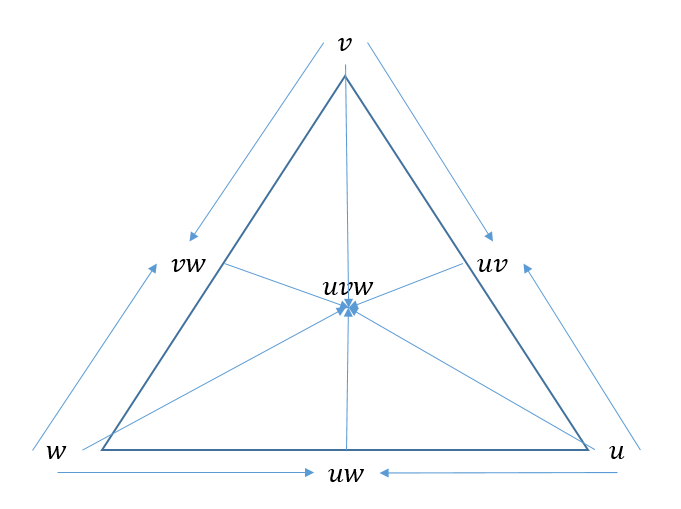
\includegraphics[scale=0.3]{images/commuting-diagram.png}
    \caption{The following diagram should commute for \(\coboundary \psi(uvw)=Id\)}
    \label{fig:commuting}
\end{figure}
See \pref{fig:commuting} for an illustration.

To state this more easily, let us introduce the flag complex.

\begin{definition}[Flag complex] \label{def:flag-complex}
Let \(X\) be a simplicial complex. The flag complex is the complex \(GX\) whose vertices are the faces of \(X\), and \(\set{s_0,s_1,...,s_k} \in GX(k)\) if \(s_0 \subset s_1 \subset ... \subset s_k\) (for some ordering of the faces).
\end{definition}
\begin{claim} \label{claim:cochains-in-flag-complex-correspondence}
    Let \(X\) be a two dimensional simplicial complex and let \(\phi \in C^1(GX,Sym(\ell))\). Let \(\psi=\psi_\phi:X(1)\to Sym(\ell)\) be given by \(\psi(uv)=\phi(uv,v)\phi(u,uv)\). Then
    %
    %
    for every triangle \(t \in X(2)\), if for all six choices of $v\in e\in t$, \(\coboundary \phi(\set{v \in e \subset t}) = Id\), then \(\coboundary \psi(t) = Id\).
\end{claim}

\begin{corollary}\torestate{\label{cor:cocycles-in-flag-complex}
    Let \(X\) be a two dimensional simplicial complex and let \(\phi \in Z^1(GX,Sym(\ell))\). Let \(\psi=\psi_\phi:X(1)\to Sym(\ell)\) be given by \(\psi(uv)=\phi(uv,v)\phi(u,uv)\). Then  \(\psi \in Z^1(X,Sym(\ell))\).}
\end{corollary}

\begin{proof}[Proof of \pref{claim:cochains-in-flag-complex-correspondence}]
    The proof is just a calculation. Let \(uvw \in X(2)\) be a triangle. We need to show that \(\psi(wv)\circ \psi(uw)=\psi(uv)\). Note that
    \[\psi(uv)=\phi(uv,v)\phi(u,uv) = \phi(uv,v)\left [\phi(uvw,uv) \phi(uv,uvw) \right ] \phi(u,uv) = \phi(uvw,v)\phi(u,uvw).\]
    Where the last equality follows from \(\coboundary \phi(u,uv,uvw)=Id\) so \(\phi(uv,uvw) \phi(u,uv)=\phi(u,uvw)\) and \(\phi(uv,v)\phi(uvw,uv)=\phi(uvw,v)\).
    Similarly, we have that 
    \begin{equation}
        \psi(uw)=\phi(uvw,w)\phi(u,uvw); \; \psi(wv)=\phi(uvw,v)\phi(w,uvw).
    \end{equation}
    Thus,
    \begin{align*}
        \psi(uv) &= \phi(uvw,v)\phi(u,uvw)\\
        &=\phi(uvw,v)\left [ \phi(w,uvw) \phi(uvw,w) \right ]\phi(u,uvw)\\
        &=\left [\phi(uvw,v) \phi(w,uvw)\right ]\cdot  \left [\phi(uvw,w) \phi(u,uvw)\right ] \\
        &= \psi(wv)\psi(uw).
    \end{align*}
\end{proof}

\subsection{Swap cosystolic expansion and the Faces complex}
For any simplicial complex $X$, we define a related complex called the {\em faces complex} of $X$, denoted $\FX{d_1}X$. This is a complex whose vertices are $d_1$ faces of $X$ and whose edges connect two vertices whose disjoint union is also a face of $X$. Thus, the underlying graph of $\FX{d_1}X$ is the graph of the swap walk on $X$, see \cite{AlevFT2019,DiksteinD2019}. This definition already appeared as \pref{def:face-complex-intro} but we restate it again here.

\begin{definition}[Faces Complex] \label{def:face-complex}
    Let \(X\) be a \(d\)-dimensional simplicial complex. Let \(d_1 \leq d\). We denote by \(\FX{d_1}X=F(X,d_1)\) the simplicial complex whose vertices are \(\FX{d_1}X(0)=X(d_1)\) and whose faces are all \(\sett{\set{s_0,s_1,...,s_j}}{s_0\dunion s_1 \dunion \dots \dunion s_j \in X}\). 
\end{definition}
It is easy to verify that this complex is \(\left ( \lfloor \frac{d+1}{d_1+1} \rfloor - 1 \right )\)-dimensional and that if \(X\) is a clique complex then so is \(\FX{d_1}X\). We omit \(d_1\) from the notation when it is clear. 

For a face $s\in X$ we write $\FX{d_1}X_s = \FX{d_1}(X_s)$. In case \(s \in X(d_1)\) then \(\FX{d_1}X_s\) is actually the link of \(s\) in $\FX{d_1}X$, i.e. \(\FX{d_1}(X_s) = (\FX{d_1}X)_s\), so this notation is not overloaded. We will be interested in $\FX{d_1}X_r$ for faces $r$ not necessarily in \(X(d_1)\). These are sub-complexes of $\FX{d_1}X$ that are not links per se. 


\begin{definition}[Well connected] \label{def:well-connected-complex}
    Let \(X\) be a \(d\)-dimensional simplicial complex. Let \(d_1 \leq d+2\). We say that \(X\) is \emph{\(d_1\)-well-connected} if for every \(r \in X^{\leq d_1}\) it holds that \(\FX{d_1}(X_r)=\FX{d_1}X_r\) is connected. Moreover, if \(r \in X(0)\) then we require that \(\FX{d_1}X_r\) is \emph{simply connected}. When \(d_1\) is clear from context we omit it and say that \(X\) is \emph{well connected}.
\end{definition}
%
We say that a complex $X$ has swap cosystolic expansion if $\FX{d_1}X$ is a cosystolic expander. Namely, recalling \pref{def:def-of-cosyst-exp},
\begin{definition}[Swap cosystolic expansion]\label{def:swapce}
    Let $d_1\in \mathbb{N}$ and let $\beta>0$. A simplicial complex $X$ of dimension $d>d_1$ has $(\beta,d_1)$ swap-cosystolic -expansion if $\FX{d_1}X$ is a $\beta$ cosystolic expander. We further say that $X$ has $(\beta,d_1)$ swap-coboundary-expansion if it has $(\beta,d_1)$ swap-cosystolic-expansion and furthermore, $\FX{d_1}X$ is simply connected. 
\end{definition}
%
\subsection{Sampling in HDXs}
%
\begin{theorem}[\cite{DiksteinH2023}] \label{thm:sampling-in-HDXs}
    Let \(k\leq d_1 \leq d\). Let \(\gamma < 1\) and let \(X\) be \(\frac{\gamma}{d}\)-one sided high dimensional expander. Let \(\zeta > 0\) and let \(f:X(k) \to [0,1]\). Let 
    \[B(f) = \sett{t \in X(d_1)}{\Abs{\Ex[r\in X(k), r\subseteq t]{f(r)}-\Ex[r \in X(k)]{f}} > \zeta}.\] 
    Then
    \[\Prob[t \in X(d_1)]{B(f)} \leq \exp(-\poly(\zeta) \frac{d_1}{k}).\]

    In particular, if \(A \subseteq X(k)\) and 
    \[B(A) = \sett{t \in X(d_1)}{\Abs{\cProb{r\in X(k)}{A}{r\subseteq t}-\Prob[r \in X(k)]{A}} > \zeta},\] 
    then
    \[\Prob[t \in X(d_1)]{B(A)} \leq \exp(-\poly(\zeta) \frac{d_1}{k}).\]
\end{theorem}
The ``in particular'' part follows from the case for \(f=\one_A\) the indicator of \(A\).

\pref{thm:sampling-in-HDXs} allows us to get a similar sampling guarantee on sampling of of tuples according to \(\mathcal{D}\) distributions extended to high dimensional expanders \(X\).

\begin{claim} \label{claim:edge-sampling}
    Let \(k \leq d_1 \leq d\) and \(q \in \NN\). Let \(d_1 \geq qk\) and let \(\zeta > 0\) be some constant. Let \(X\) be a \(d\)-dimensional simplicial complex as in \pref{thm:sampling-in-HDXs}. Let \(\mathcal{D}\) be an agreement distribution over \(\Delta_{qk+q}(k)\). and let \(E \subseteq \supp \mathcal{D}_X\). Then
    \[\Prob[s \in X(d_1)]{\Abs{\cProb{\set{r_i} \sim \mathcal{D}}{E}{\set{r_i} \subseteq s} - \Prob[\set{r_i} \sim D]{E}} > \zeta} \leq \exp(-\poly(\zeta) \frac{d_1}{k}).\]
\end{claim}

\begin{proof}[Proof of \pref{claim:edge-sampling}]
    Let \(f:X(qk+q-1) \to [0,1]\) be \(f(a)=\Prob[\set{r_i} \subseteq a]{E}\). Then \(\ex{f}=\prob{E}\) and \(\Ex[a \subseteq s]{f(a)} = \cProb{\set{r_i} \sim \mathcal{D}}{E}{\set{r_i} \subseteq s}\). \pref{thm:sampling-in-HDXs} gives us the claim.
\end{proof}

\subsection{Suitable complexes}
\begin{definition}[Suitable complex] \label{def:suitable-complexes}
    Let \(d>k>0\) be integers, and let \(\alpha > 0\). Let \(X\) be a \(d\)-dimensional simplicial complex. We say that \(X\) is \((d,k,\alpha)\)-\emph{suitable} if it has the following properties: 
\begin{enumerate}
    \item There exists some integer \(d_1<d\) with the following properties:
    \begin{enumerate}
        \item \(k^3 \leq d_1 \leq d \exp(-\alpha\frac{d_1}{k})\).
        \item \label{item:cob-exp} $X$ has \((\exp(-\alpha \frac{d_1}{k}),d_1)\)-swap-cosystolic expansion, as in \pref{def:swapce}. 
        \item \label{item:well-connected} \(X\) is \(d_1\)-well connected as in \pref{def:well-connected-complex}.
    \end{enumerate}
    \item \(X\) is a \(\frac{1}{d^2}\)-two-sided local spectral expander.
    \item \(X\) is a clique complex. 
    \end{enumerate}
We also say that $X$ is suitable with respect to $d_1$.
\end{definition}

These properties are abstract and a priori it is not clear whether there is a complex that satisfies them, especially the property of the face complex being a coboundary expander. However, the following two families of complexes satisfy all of these properties.
\begin{example}~
    \begin{enumerate}
    \item The \(SL_d(\mathbb{F}_q)\)-spherical building (see \pref{def:sph-bldg}) for sufficiently large prime power \(q\) and dimension \(d\). 
    \item \cite{LubotzkySV2005b} complexes, that are connected simplicial complexes whose links look like the spherical buildings in the first item.
\end{enumerate}
\end{example}

\begin{theorem}[Based on \cite{DiksteinD2023b}] \label{thm:spherical-building-and-LSV-complexes-are-suitable}
Let \(d,k,\alpha\) be such that \(\alpha \in (0,1)\) and \(d \geq \poly(k,\alpha)\). Then there exists a constant \(q_0=q_0(k,\alpha)\) such that for every prime power \(q>q_0\):
    \begin{enumerate}
        \item The \(SL_{d}(\mathbb{F}_q)\)-spherical building is a \((d,k,\alpha)\)-\emph{suitable}.
        \item \(d\)-dimensional \cite{LubotzkySV2005b} complexes, such that the link of every vertex is isomorphic to \(SL_{d-1}(\mathbb{F}_q)\)-spherical building are \((d,k,\alpha)\)-suitable. 
    \end{enumerate}
\end{theorem}
This paper is focused on the \(1\%\)-agreement theorem; the proof of swap cosystolic expansion gives rise to other significant challenges so we defer the proof of the swap cosystolic expansion to a companion paper \cite{DiksteinD2023b}.

\begin{proof}
In both cases we fix \(k\) and take \(d_1 = k^3\).
\begin{enumerate}
\item \begin{enumerate}
        \item\textbf{Swap-coboundary and cosystolic expansion.} This is the main theorem in \cite{DiksteinD2023b}, which shows that \(F{d_1}X\) is a \(\exp(-\Omega(\sqrt{d_1})\)-cosystolic expander for these complexes (a coboundary expander in the spherical building case).
        \item\textbf{Well connectedness.} Let \(s\) be a face in a complex \(X\) (which is one of the complexes in the theorem). Then \((\FX{d_1}X)_s = \FX{d_1}(X_s)\). In both cases, this is (isomorphic to) a faces complex of a link in the spherical building. In particular, \cite{DiksteinD2023b} shows that these are coboundary expanders - a strictly stronger property than simple connectivity.
\end{enumerate}
    \item\textbf{high dimensional expansion.} High dimensional expansion of the spherical buildings decays with \(q\). This bound is independent of the ambient dimension, as proven in \cite{AbdolazimiO2022}. Therefore there is a sufficiently large enough \(q\) such that the spherical building is a \(\frac{1}{d^2}\)-high dimensional expander. High dimensional expansion of the \cite{LubotzkySV2005b} complexes follows from the fact that their links are spectral expanders and \pref{thm:trickle-down} by \cite{Oppenheim2018}.
    \item\textbf{Clique complexes.} It is easy to show that the spherical building is a clique complex by definition. If \(\set{u_0,u_1,\dots,u_k}\) are such that all edges appear in the spherical building, it means that every two subspaces are contained in one another. Rearranging them by dimension shows that this in indeed a flag, i.e. a face in the spherical building. The fact that quotients of the spherical buildings are clique complexes appear e.g. in \cite{LubotzkySV2005a}. 

\end{enumerate}
\end{proof}

